% INTRODUCCIÓN

\cleardoublepage

\chapter{Retrievers}

\section{Introducción}

Habiendo introducido los conceptos fundamentales de los Modelos de Lenguaje a Gran Escala (LLMs) y los RAG en los capítulos anteriores, ahora nos centramos en uno de los componentes críticos que potencian los sistemas RAG: los \textit{retrievers}. Este concepto es esencial para la creación de un RAG sobre un LLM, permitiéndole acceder a información actualizada y relevante más allá de su entrenamiento inicial.

En este capítulo, exploraremos los diferentes tipos de \textit{retrievers}, cómo se integran en los sistemas RAG y las distintas metodologías para su implementación. Discutiremos desde los simples \textit{retrievers} basados en bases de datos vectoriales hasta complejas configuraciones que involucran múltiples métodos de recuperación de información.

\section{Fundamentos de los Retrievers}

\subsection{Definición y Función}

Un \textit{retriever} es una herramienta que busca y recupera información relevante de un conjunto de datos grande y posiblemente no estructurado. En el contexto de RAG, un \textit{retriever} actúa como el puente entre la pregunta del usuario y la base de conocimientos o información almacenada. La eficacia de un \textit{retriever} es crucial, ya que determina la calidad y la relevancia de la información que se utiliza para generar respuestas.

\subsection{Rol en RAG}

Como se puede ver en la figura \ref{fig:retriever}, en un sistema RAG, el retriever selecciona fragmentos de texto o documentos que son potencialmente útiles para responder a una consulta específica. Estos documentos se pasan luego a un modelo de lenguaje, que integra esta información para generar una respuesta coherente y contextualmente rica. Esta capacidad de incorporar información dinámica de diversas fuentes externas distingue a los RAGs de los modelos de lenguaje tradicionales que dependen únicamente de lo que han aprendido durante su entrenamiento inicial.

\begin{figure}[h]
\centering
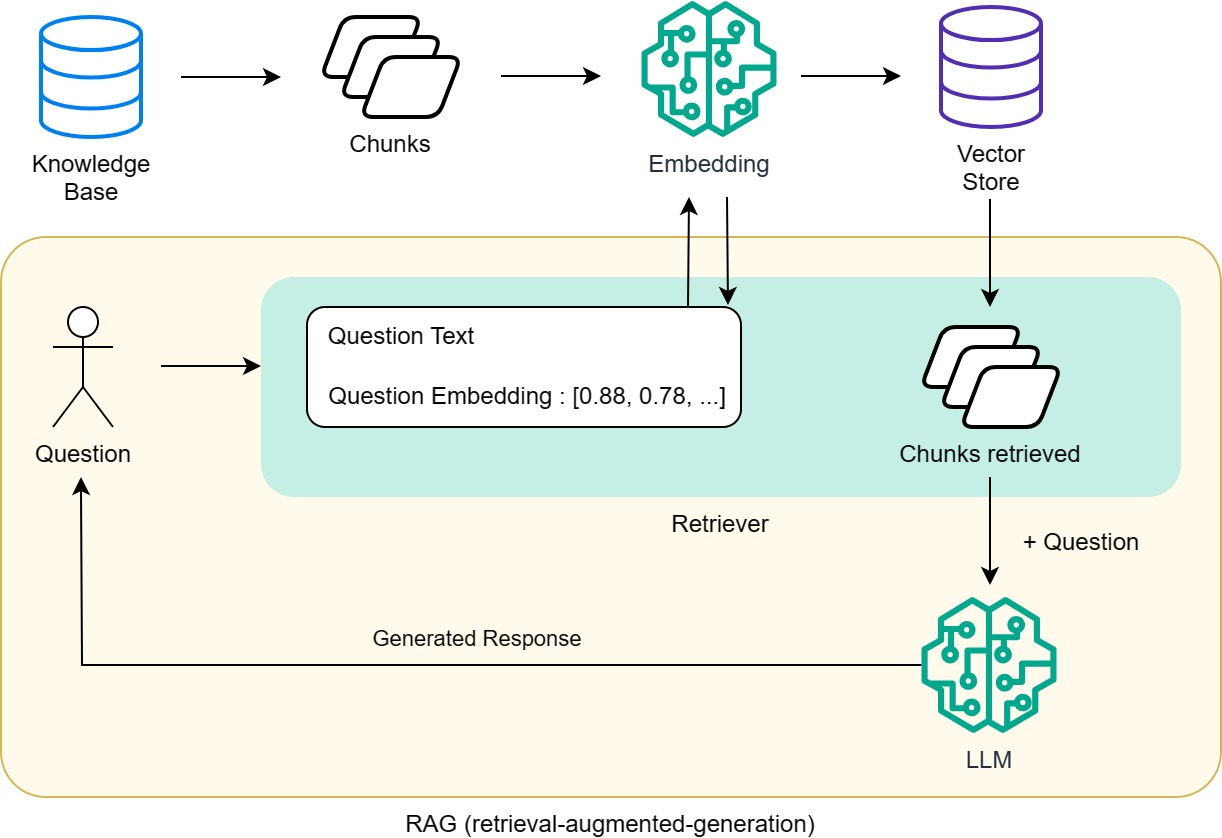
\includegraphics[width=0.8\textwidth]{figuras/capitulo5/retriever.jpg}
\caption{Esquema de un RAG}
\label{fig:retriever}
\end{figure}

\section{Tipos de Retrievers Tradicionales}

Los retrievers se clasifican principalmente en tres tipos, cada uno con sus propias técnicas y aplicaciones preferidas en el procesamiento de consultas y la recuperación de información. Estos son los retrievers \textit{sparse}, \textit{dense} e \textit{hybrid}.

\subsection{Retrievers Sparse}

Los retrievers \textit{sparse} utilizan métodos basados en coincidencia de términos para recuperar documentos. Estos métodos, como TF-IDF (Frequency-Inverse Document Frequency) y BM25, analizan la frecuencia de las palabras en documentos para determinar su relevancia con respecto a una consulta. La principal ventaja de los retrievers sparse es su eficiencia y rapidez, lo que los hace adecuados para grandes volúmenes de datos donde la relevancia se puede medir por la presencia de palabras clave específicas. \citep{lewis2020retrieval}

Estos retrievers son particularmente útiles en situaciones donde las consultas son directas y las palabras clave bien definidas son suficientes para recuperar información relevante. Sin embargo, pueden no ser efectivos en contextos donde la semántica de la consulta es más importante que las palabras específicas utilizadas.

\subsection{Retrievers Dense}

Por otro lado, los retrievers \textit{dense} emplean modelos de vectorización (embeddings) para representar tanto las consultas como los documentos como vectores densos en un espacio vectorial continuo. Estos modelos capturan la semántica de las palabras y las frases, permitiendo una recuperación más efectiva en casos donde las consultas y los documentos no comparten términos exactos pero están relacionados en contexto y significado. \citep{lewis2020retrieval}

Los retrievers dense son esenciales para aplicaciones donde la relevancia semántica entre la consulta y los documentos es más crítica que la coincidencia exacta de palabras. Su capacidad para entender y procesar el lenguaje de manera más natural los hace muy valiosos en sistemas RAG modernos. Estos retrievers son muy dependientes del modelo de vectorización usado.

\subsection{Retrievers Hybrid}

Finalmente, los retrievers \textit{hybrid} combinan las técnicas de los retrievers sparse y dense para aprovechar las ventajas de ambos. Este enfoque permite una recuperación inicial rápida de documentos potencialmente relevantes utilizando métodos sparse, seguida de un refinamiento más detallado y semánticamente rico con técnicas dense.

Los retrievers hybrid ofrecen un equilibrio entre eficiencia y profundidad semántica, lo que los hace ideales para sistemas RAG que requieren tanto precisión en la recuperación de información relevante como la capacidad de manejar grandes volúmenes de datos.

Cada tipo de retriever tiene su lugar en el ecosistema de los RAG, y la elección de uno sobre otro depende en gran medida de las necesidades específicas del sistema y las características de las consultas y los conjuntos de datos utilizados.

\section{Retrievers Avanzados}

Dada la evolución constante de los sistemas RAG y la necesidad de integrar información más específica y contextual, la comunidad ha estado desarrollando diferentes retrievers que tienen sentido en determinados contextos. Estos retrievers utilizan técnicas sofisticadas para mejorar la precisión y la relevancia de la información recuperada. Aquí exploramos varios enfoques que se recopilan en la web de langchain \citep{langchainretrievers}.

\subsection{Documento Matriz (Parent Document)}

Este tipo de retriever es ideal cuando los documentos contienen numerosos fragmentos de información distintos que se benefician de ser indexados individualmente, pero que es preferible recuperar juntos. El proceso involucra la indexación de múltiples fragmentos o trozos de cada documento. Luego, estos fragmentos se buscan en el espacio de vectores (embeddings) para identificar aquellos que son más similares entre sí, pero en lugar de recuperar solo los fragmentos individuales, se recupera y devuelve el documento completo al que pertenecen. Esta metodología asegura que toda la información contextual relacionada esté disponible para generar respuestas más completas y detalladas.

\subsubsection{Multi Vector}

Este retriever es especialmente útil cuando es posible extraer de los documentos información que se considera relevante para indexar (a parte del texto en sí). El proceso implica la creación de múltiples vectores para cada documento. Cada vector puede ser generado de diversas maneras, incluyendo, por ejemplo, resúmenes del texto, preguntas hipotéticas, descripciones de imágenes o tablas, etc. 
Esta técnica permite una representación más rica de los documentos, facilitando una recuperación más precisa y alineada con las necesidades específicas del retriever.


\subsection{Consulta Autónoma (Self Query)}

Utiliza un LLM para transformar la entrada del usuario en dos componentes principales: una cadena que se busca semánticamente y un filtro de metadatos que acompaña la consulta. Este método es particularmente valioso porque muchas veces las preguntas están relacionadas con los metadatos de los documentos, no con su contenido textual directo. La capacidad de enfocar la búsqueda en metadatos permite recuperar información que es más relevante para la intención específica del usuario, mejorando así la precisión y utilidad de las respuestas generadas. Este tipo de retriever es especialmente útil cuando las preguntas de los usuarios se responden mejor recuperando documentos basados en metadatos en lugar de en similitudes textuales directas

\begin{figure}[h]
\centering
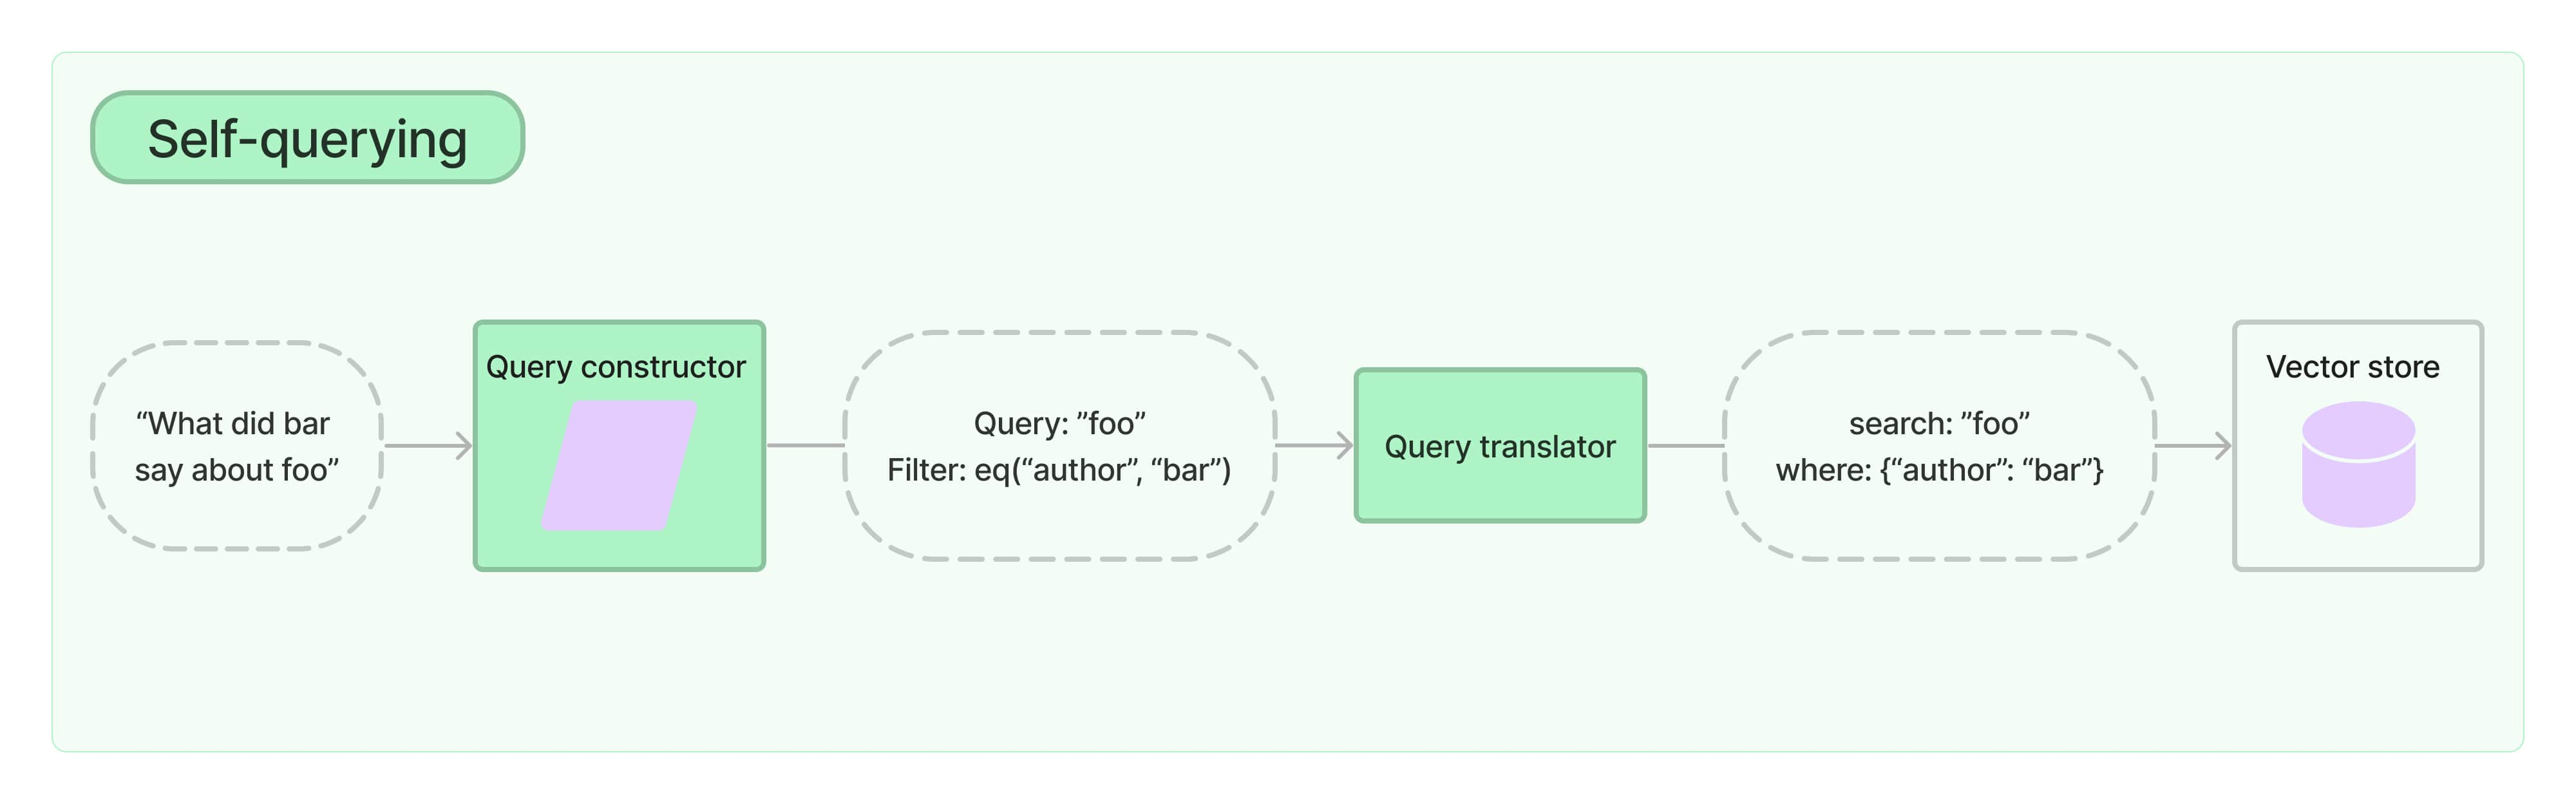
\includegraphics[width=0.8\textwidth]{figuras/capitulo5/self_query.jpg}
\caption{Esquema de un Self Query retriever \citep{langchainretrievers}}
\label{fig:retrieverselfquery}
\end{figure}


\subsubsection{Compresión Contextual}

Uno de los desafíos en la recuperación de documentos es que generalmente no se conocen las consultas específicas que enfrentará el sistema de almacenamiento de documentos cuando se ingieren datos en el sistema. Esto significa que la información más relevante para una consulta puede estar enterrada en un documento con mucho texto irrelevante. Pasar ese documento completo a través de la aplicación puede llevar a llamadas más costosas al LLM y a respuestas de menor calidad.

La compresión contextual está diseñada para solucionar esto. En lugar de devolver inmediatamente los documentos recuperados tal como están, se pueden comprimir utilizando el contexto de la consulta dada, de modo que solo se devuelva la información relevante.


\subsection{Time-Weighted Vectorstore}

Optimiza la recuperación basándose tanto en la similitud semántica como en la fechateams del documento. Es ideal para aplicaciones donde la información más actual es crucial, como en el seguimiento de noticias o tendencias del mercado.

\subsection{Multi-Query Retriever}

Genera múltiples consultas a partir de una inicial para abordar consultas complejas que requieren información sobre varios temas. Luego, recupera documentos para cada una de estas consultas, lo que garantiza una respuesta exhaustiva y detallada. Es muy útil cuando las preguntas van a tratar sobre varios temas y temas no relacionados.

\subsection{Long-Context Reorder}

Es especialmente útil en modelos que enfrentan degradaciones de rendimiento cuando deben acceder a información relevante en medio de contextos extensos. Este tipo de retriever reordena los documentos recuperados para optimizar la atención del modelo a la información más pertinente, colocando los documentos más relevantes al principio y al final, mientras que los menos relevantes quedan en el medio.
El "Long Context Reorder" utiliza un enfoque específico conocido como "Lost in the middle" para contrarrestar el problema de que los modelos ignoren documentos importantes simplemente porque aparecen en posiciones menos destacadas dentro de un conjunto de datos grande. \citep{liu2023lost}

Estos retrievers avanzados representan un conjunto diverso de herramientas diseñadas para mejorar la eficiencia y efectividad de los sistemas RAG, facilitando respuestas más precisas y contextuales en una amplia variedad de aplicaciones.

\section{Conclusión}

A lo largo de este capítulo, hemos explorado en profundidad los diversos tipos de \textit{retrievers} que potencian los sistemas de RAG. Hemos visto cómo los \textit{retrievers} no solo facilitan la recuperación de información relevante y actualizada, sino que también optimizan la eficiencia del procesamiento y la precisión de las respuestas generadas por los LLMs. La implementación adecuada de estos \textit{retrievers} puede marcar una diferencia significativa en la capacidad de un sistema RAG para proporcionar respuestas precisas, contextuales y de alta calidad.

Este capítulo también ha subrayado la importancia de elegir el tipo correcto de \textit{retriever} según las necesidades específicas del sistema y del dominio de aplicación. Con las tecnologías emergentes y los desarrollos continuos en el campo de la inteligencia artificial, es probable que veamos aún más innovaciones en los métodos de recuperación, lo que a su vez podría ampliar aún más las capacidades y aplicaciones de los RAGs.

En resumen, los \textit{retrievers} son componentes cruciales que no solo enriquecen la funcionalidad de los sistemas basados en LLMs mediante la incorporación de conocimientos actualizados y contextualmente relevantes, sino que también representan un área de investigación activa y en evolución que continuará influyendo en el futuro de la generación de lenguaje y la recuperación de información.





